\chapter{الهواء خليط من الغازات}\label{ch:g4:air-a-mixture-of-gases}

في يوم عاصف تشد الطائرة الورقية خيطها، وعلى البحيرة يمتلئ الشراع ويدفع
القارب إلى الأمام. ثمة شيء يدفعهما، ومع ذلك لا نرى شيئًا. هذا الشيء هو
\omterm{def:g4:air-a-mixture-of-gases:air}{الهواء}. لا نستطيع أن نراه، لكنه في كل مكان من حولنا، يملأ كل قارورة
فارغة وكل غرفة، وندخله إلى أجسامنا مع كل نفس. فمِمَّ يتكون \omterm{def:g4:air-a-mixture-of-gases:air}{الهواء}؟

\begin{recall}
\omterm{def:g2:mixing-and-dissolving:mix}{الخلط} أن نضع أشياء مختلفة معًا؛ وما نحصل عليه خليط من هذه الأشياء،
ولا يضيع شيء حين نخلطها
(\cref{ch:g2:mixing-and-dissolving}).
\end{recall}

\begin{omfigure}
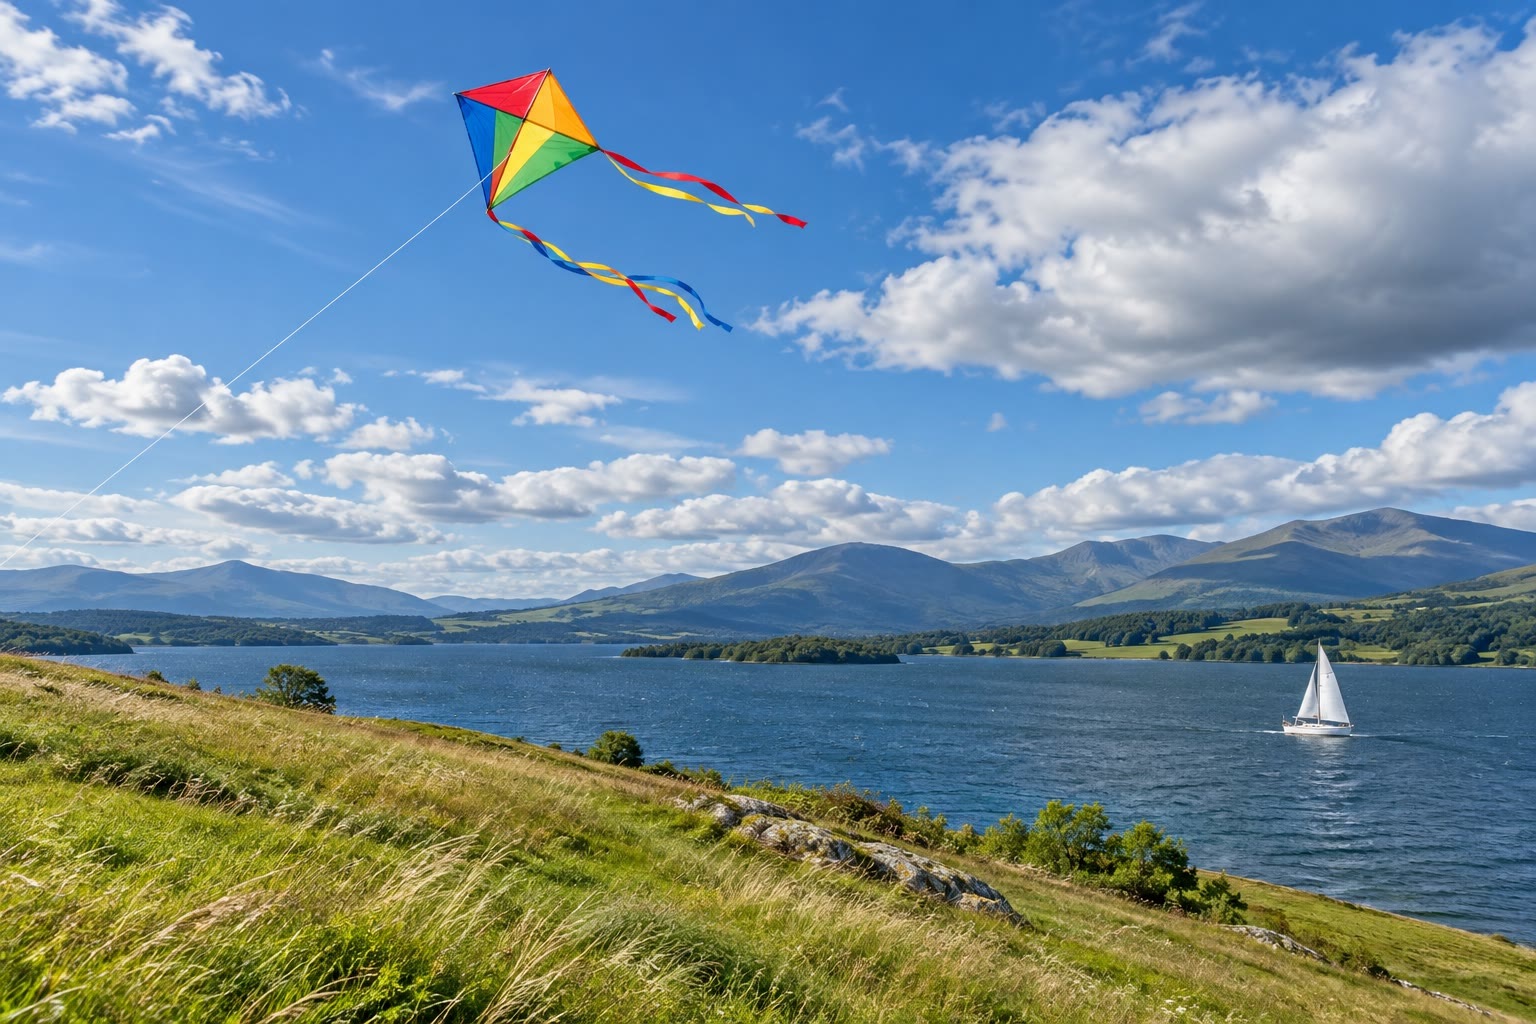
\includegraphics[width=0.6\linewidth]{images/book1/ai/g4-kite-day.jpg}

{\small طائرة ورقية وشراع: \omterm{def:g4:air-a-mixture-of-gases:air}{الهواء} لا يُرى، لكنه يدفع.}
\end{omfigure}

\section{الهواء في كل مكان من حولنا}

\begin{example}[كأس مقلوبة]\label{ex:g4:air-a-mixture-of-gases:glass}
نضغط منديلًا ورقيًا جافًا في قاع كأس فارغة. ثم نقلب الكأس وندفعها
مستقيمة إلى الأسفل في وعاء ماء. وحين نرفعها من جديد نجد المنديل لا يزال
جافًا. لم تكن الكأس فارغة: كانت مملوءة \omterm{def:g4:air-a-mixture-of-gases:air}{بالهواء}، \omterm{def:g4:air-a-mixture-of-gases:air}{والهواء} منع الماء من
الدخول.
\end{example}

\begin{omfigure}
\begin{tikzpicture}[font=\small, scale=1.3]
  \pic[transform shape] at (0,0) {trough};
  % the upturned glass, rim at y = 0.35, base at y = 2.35
  \fill[white] (-0.8,0.5) rectangle (0.8,0.95);
  \pic[transform shape, rotate=180] at (0,2.35) {beaker={0}{white}};
  % the tissue at the top, inside
  \fill[white, draw=black!45, rounded corners=1.5pt] (-0.4,2.33) -- (-0.3,2.05)
    -- (-0.1,2.12) -- (0.05,1.98) -- (0.25,2.1) -- (0.42,2.02) -- (0.45,2.33) -- cycle;
  \draw[<-, omProp, thick] (0.45,2.12) -- (2.4,2.5) node[right, text=black]
    {منديل جاف};
  \draw[<-, omProp, thick] (0.3,1.2) -- (2.4,1.4) node[right, text=black]
    {الهواء: يمنع الماء من الدخول};
  \draw[<-, omProp, thick] (1.4,0.7) -- (2.4,0.55) node[right, text=black]
    {الماء};
\end{tikzpicture}

{\small تُدفع الكأس مقلوبة في الماء. فيمنع \omterm{def:g4:air-a-mixture-of-gases:air}{الهواء} المحبوس فيها الماء من
الدخول، ويبقى المنديل جافًا.}
\end{omfigure}


\begin{remark}[الهواء غاز]\label{rem:g4:air-a-mixture-of-gases:gas}
\omterm{def:g4:air-a-mixture-of-gases:air}{الهواء} غاز: ليس له شكل خاص به، وينتشر ليملأ أي وعاء. وهو مع ذلك
مادة، فالبالون المملوء \omterm{def:g4:air-a-mixture-of-gases:air}{بالهواء} أثقل قليلًا من البالون نفسه فارغًا. أما
ما هي الغازات، ولماذا تسلك هذا السلوك، فيرويه كتاب الفيزياء.
\end{remark}

\section{الهواء خليط}

\begin{definition}[الهواء]\label{def:g4:air-a-mixture-of-gases:air}
\emph{الهواء}\index{هواء} خليط الغازات الذي يحيط بالأرض. وهو ليس غازًا
واحدًا: بل تختلط فيه عدة غازات، ويمكن أن يُفصل بعضها عن
بعض.
\end{definition}

\begin{proposition}[مِمَّ يتكون الهواء]\label{prop:g4:air-a-mixture-of-gases:composition}
% ledger: air:N2, air:O2, air:Ar, air:trace, air:CO2, air:H2O
إذا تركنا جانبًا بخار الماء الذي فيه، \omterm{def:g4:air-a-mixture-of-gases:air}{فالهواء} يتكون من:
\begin{itemize}
  \item \textbf{النيتروجين}، نحو أربعة أخماس \omterm{def:g4:air-a-mixture-of-gases:air}{الهواء}؛
  \item \textbf{الأكسجين}، نحو خمس \omterm{def:g4:air-a-mixture-of-gases:air}{الهواء}؛
  \item قليل من \textbf{الأرغون}، نحو جزء واحد من 100؛
  \item قليل جدًا من \textbf{ثنائي أكسيد الكربون}، نحو 4 أجزاء من 10\,000،
        ومقادير ضئيلة من غازات أخرى.
\end{itemize}
ويحمل \omterm{def:g4:air-a-mixture-of-gases:air}{الهواء} أيضًا \textbf{بخار الماء}، وهو لا يُرى: قليلًا جدًا في يوم
بارد جاف، وحتى نحو 4 أجزاء من 100 في يوم حار رطب.
\end{proposition}

\begin{example}[مئة قارورة من الهواء]\label{ex:g4:air-a-mixture-of-gases:hundred}
% ledger: air:N2, air:O2, air:Ar
تخيّل 100 قارورة من \omterm{def:g4:air-a-mixture-of-gases:air}{الهواء} الجاف، وقد فُرزت غازات \omterm{def:g4:air-a-mixture-of-gases:air}{الهواء} في قوارير
منفصلة. فنحو 78 قارورة تحوي النيتروجين، و21 قارورة الأكسجين، والقارورة
الأخيرة الأرغون، ومعه ما يعادل بضع قطرات من ثنائي أكسيد الكربون
وغازات أخرى.
\end{example}

\begin{omfigure}
\begin{tikzpicture}[font=\small, x=0.42cm, y=0.42cm]
  \foreach \k in {0,...,99} {
    \pgfmathtruncatemacro\col{mod(\k,10)}
    \pgfmathtruncatemacro\row{9-int(\k/10)}
    \ifnum\k<78 \def\c{omDef!45}\else\ifnum\k<99 \def\c{red!45}\else\def\c{cyan!60}\fi\fi
    \fill[\c, draw=white, line width=0.8pt] (\col,\row) rectangle ++(1,1);
  }
  \fill[omDef!45] (12,8) rectangle ++(1,1);
  \node[anchor=west] at (13.3,8.5) {\foreignlanguage{arabic}{النيتروجين: \babelsublr{78} مربعًا}};
  \fill[red!45] (12,6) rectangle ++(1,1);
  \node[anchor=west] at (13.3,6.5) {\foreignlanguage{arabic}{الأكسجين: \babelsublr{21} مربعًا}};
  \fill[cyan!60] (12,4) rectangle ++(1,1);
  \node[anchor=west, align=left] at (13.3,4.5) {الأرغون وثنائي أكسيد الكربون\\ والباقي: مربع واحد};
\end{tikzpicture}

{\small مئة مربع من \omterm{def:g4:air-a-mixture-of-gases:air}{الهواء} الجاف. المربع الذي في أسفل اليمين يحوي
الأرغون، وثنائي أكسيد الكربون أصغر من أن يُرسم وحده.}
\end{omfigure}

\begin{remark}[أسماء الغازات]\label{rem:g4:air-a-mixture-of-gases:names}
النيتروجين والأكسجين والأرغون وثنائي أكسيد الكربون أسماء غازات. كلها
عديمة اللون ولا رائحة لها. وسيبيّن فصل لاحق مِمَّ يتكون كل منها، وصولًا
إلى الجسيمات الدقيقة التي تتكون منها كل المادة.
\end{remark}

\section{ما نستنشقه وما نزفره}

\begin{proposition}[هواء الزفير]\label{prop:g4:air-a-mixture-of-gases:breath}
% ledger: breath:O2, breath:CO2, breath:N2, air:O2, air:CO2
\omterm{def:g4:air-a-mixture-of-gases:air}{الهواء} الذي نزفره ليس هو \omterm{def:g4:air-a-mixture-of-gases:air}{الهواء} الذي استنشقناه. فجسمنا يأخذ بعض
الأكسجين ويطرح ثنائي أكسيد الكربون وبخار الماء:
\begin{itemize}
  \item نحو 21 جزءًا من 100 من \omterm{def:g4:air-a-mixture-of-gases:air}{هواء} الشهيق أكسجين، لكن نحو 16 جزءًا
        من 100 فقط من \omterm{def:g4:air-a-mixture-of-gases:air}{هواء} الزفير؛
  \item يرتفع ثنائي أكسيد الكربون من نحو 4 أجزاء من 10\,000 إلى نحو 4
        أجزاء من 100: أي نحو مئة مرة أكثر؛
  \item ونزفر النيتروجين كما استنشقناه تمامًا.
\end{itemize}
\end{proposition}

\begin{omfigure}
\begin{tikzpicture}
\begin{axis}[ybar, width=0.8\linewidth, height=5.2cm, bar width=12pt,
    ymin=0, ymax=90, ylabel={\foreignlanguage{arabic}{جزء من \babelsublr{100}}},
    symbolic x coords={nitrogen, oxygen, carbon dioxide}, xtick=data,
    xticklabels={النيتروجين, الأكسجين, ثنائي أكسيد الكربون},
    tick label style={font=\small}, label style={font=\small},
    xticklabel style={text height=1.6ex, text depth=0.4ex},
    legend style={font=\small, at={(0.98,0.95)}, anchor=north east},
    nodes near coords, nodes near coords style={font=\footnotesize},
    enlarge x limits=0.25, axis lines*=left, ymajorgrids,
    grid style={gray!20}]
% ledger: air:N2, air:O2, air:CO2, breath:N2, breath:O2, breath:CO2 (rounded)
\addplot[fill=omDef!45, draw=omDef] coordinates
  {(nitrogen,78) (oxygen,21) (carbon dioxide,0)};
\addplot[fill=omProp!55, draw=omProp] coordinates
  {(nitrogen,78) (oxygen,16) (carbon dioxide,4)};
\legend{{الشهيق}, {الزفير}}
\end{axis}
\end{tikzpicture}

{\small \omterm{def:g4:air-a-mixture-of-gases:air}{هواء} الشهيق \omterm{def:g4:air-a-mixture-of-gases:air}{وهواء} الزفير، بالأجزاء من 100 (دون بخار الماء،
والأعداد مقرّبة). أما ثنائي أكسيد الكربون في \omterm{def:g4:air-a-mixture-of-gases:air}{هواء} الشهيق، 4 أجزاء
من 10\,000، فأصغر من أن يظهر عمودًا.}
\end{omfigure}

\begin{example}[غرفة مزدحمة]\label{ex:g4:air-a-mixture-of-gases:room}
في قاعة صغيرة نوافذها مغلقة يزفر ثلاثون شخصًا ثنائي أكسيد الكربون طوال
الصباح. فيقل الأكسجين في \omterm{def:g4:air-a-mixture-of-gases:air}{هواء} الغرفة شيئًا فشيئًا ويكثر ثنائي أكسيد
الكربون، ويشعر الناس بالتعب. وفتح النوافذ يُدخل \omterm{def:g4:air-a-mixture-of-gases:air}{الهواء} النقي من
جديد.
\end{example}

\begin{omfigure}
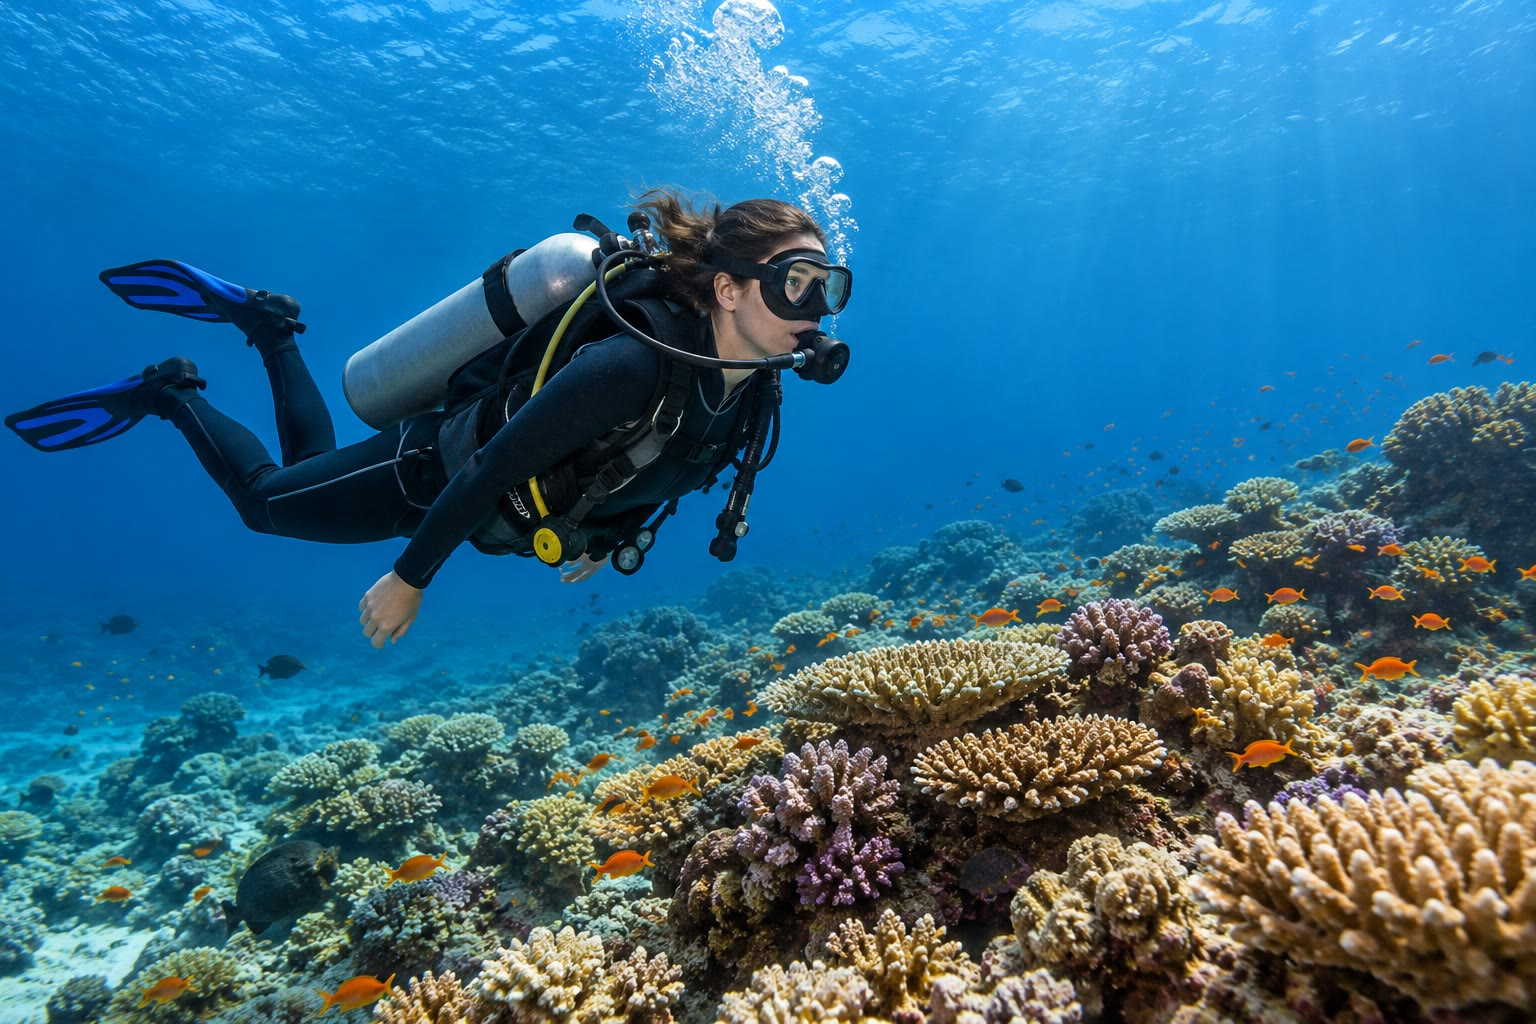
\includegraphics[width=0.55\linewidth]{images/book1/ai/g4-scuba-diver.jpg}

{\small غوّاص يتنفس \omterm{def:g4:air-a-mixture-of-gases:air}{الهواء} من القارورة التي على ظهره؛ والفقاعات هي
\omterm{def:g4:air-a-mixture-of-gases:air}{هواء} الزفير.}
\end{omfigure}

\begin{remark}[لماذا يتنفس الغواصون الهواء]\label{rem:g4:air-a-mixture-of-gases:diver}
تُملأ قارورة الغواص \omterm{def:g4:air-a-mixture-of-gases:air}{بهواء} مضغوط في حيز صغير، لا بأكسجين نقي: فتنفس
الأكسجين النقي في الأعماق خطر. والنيتروجين الذي في \omterm{def:g4:air-a-mixture-of-gases:air}{الهواء} موجود ليخفف
الأكسجين.
\end{remark}

\section{الأكسجين للحياة وللنار}

\begin{proposition}[الكائنات الحية واللهب تستهلك الأكسجين]\label{prop:g4:air-a-mixture-of-gases:oxygen}
من بين غازات \omterm{def:g4:air-a-mixture-of-gases:air}{الهواء} كلها، الأكسجين هو الذي تحتاج إليه الكائنات الحية
واللهب. فالحيوانات والناس يأخذونه حين يتنفسون؛ واللهب يأخذه من \omterm{def:g4:air-a-mixture-of-gases:air}{الهواء}
المحيط به. أما النباتات الخضراء فتعيد الأكسجين إلى \omterm{def:g4:air-a-mixture-of-gases:air}{الهواء} في ضوء
النهار.
\end{proposition}

\begin{inthelab}[شمعة تحت ناقوس]
يشعل المعلم شمعة على بلاطة ويُنزل فوقها ببطء ناقوسًا زجاجيًا كبيرًا.
فيصغر اللهب ويرتعش ثم ينطفئ بعد بضع ثوانٍ: \omterm{def:g4:air-a-mixture-of-gases:air}{فالهواء} حول اللهب لم يعد
يحوي ما يكفي من الأكسجين ليبقيه مشتعلًا. وتحت ناقوس أكبر بمرتين تشتعل
الشمعة نحو ضعف المدة، لأن فيه نحو ضعف \omterm{def:g4:air-a-mixture-of-gases:air}{الهواء}، وبالتالي ضعف الأكسجين
الذي يُستهلك.
\end{inthelab}

\begin{omfigure}
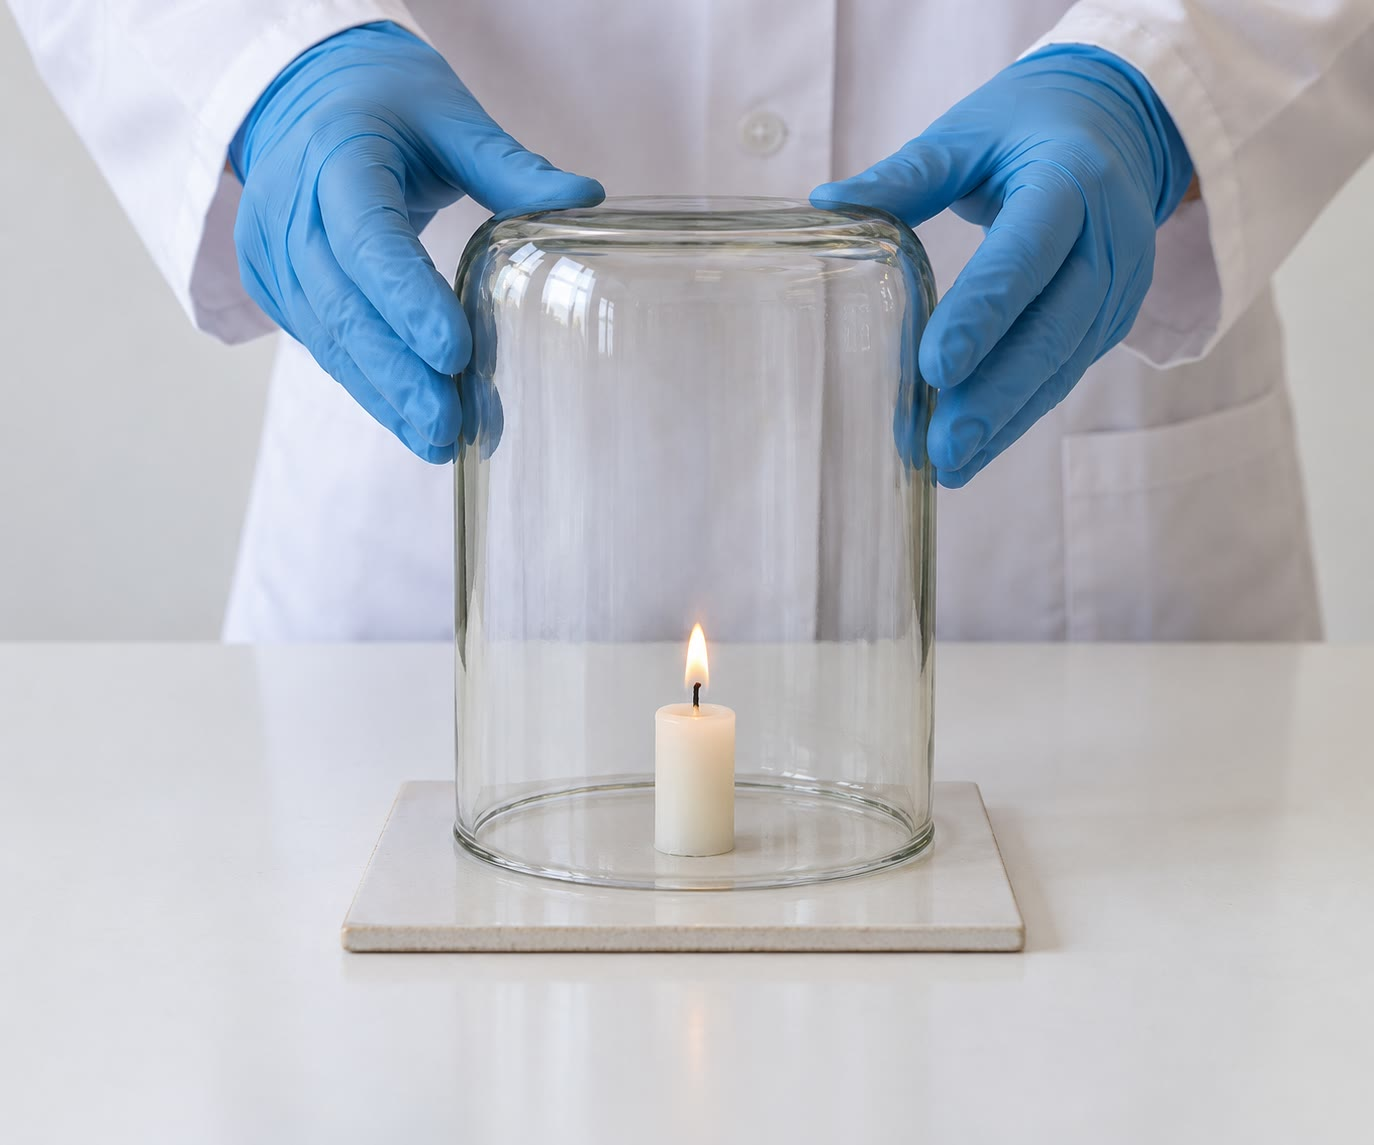
\includegraphics[width=0.5\linewidth]{images/book1/ai/g4-candle-jar-lab.jpg}

{\small شمعة تحت ناقوس زجاجي تنطفئ حين يبقى حول لهبها أكسجين
قليل جدًا.}
\end{omfigure}

\begin{remark}[النيتروجين لا يحترق]\label{rem:g4:air-a-mixture-of-gases:nitrogen}
النيتروجين هو الجزء الأكبر من \omterm{def:g4:air-a-mixture-of-gases:air}{الهواء}، ومع ذلك فهو لا يبقي اللهب مشتعلًا
ولا يستهلكه جسمنا. ولو كان \omterm{def:g4:air-a-mixture-of-gases:air}{الهواء} كله نيتروجينًا لما استطعنا أن نتنفس،
ولما احترق شيء.
\end{remark}

\section{تمارين}

\begin{exercise}[$\star$]\label{exo:g4:air-a-mixture-of-gases:1}
هل \omterm{def:g4:air-a-mixture-of-gases:air}{الهواء} غاز واحد أم خليط؟ سمِّ الغازين الرئيسيين في \omterm{def:g4:air-a-mixture-of-gases:air}{الهواء}.
\end{exercise}

\begin{exercise}[$\star$]\label{exo:g4:air-a-mixture-of-gases:2}
ما الكسر الذي يمثله النيتروجين من \omterm{def:g4:air-a-mixture-of-gases:air}{الهواء} تقريبًا؟ وما الكسر الذي يمثله
الأكسجين تقريبًا؟
\end{exercise}

\begin{exercise}[$\star$]\label{exo:g4:air-a-mixture-of-gases:3}
في 100 لتر من \omterm{def:g4:air-a-mixture-of-gases:air}{الهواء} الجاف، كم لترًا من النيتروجين تقريبًا؟ وكم لترًا من
الأكسجين تقريبًا؟
\end{exercise}

\begin{exercise}[$\star$]\label{exo:g4:air-a-mixture-of-gases:4}
نضع قارورة فارغة مقلوبة في حوض ماء. لماذا لا يملأ الماء
القارورة؟
\end{exercise}

\begin{exercise}[$\star$]\label{exo:g4:air-a-mixture-of-gases:5}
انظر إلى المخطط بالأعمدة. أي غاز يقل في \omterm{def:g4:air-a-mixture-of-gases:air}{هواء} الزفير؟ وأي غاز
يزيد؟
\end{exercise}

\begin{exercise}[$\star$]\label{exo:g4:air-a-mixture-of-gases:6}
أي غاز من غازات \omterm{def:g4:air-a-mixture-of-gases:air}{الهواء} يحتاج إليه اللهب؟ وأي غاز من غازات \omterm{def:g4:air-a-mixture-of-gases:air}{الهواء} نحتاج
إليه حين نتنفس؟
\end{exercise}

\begin{exercise}[$\star$]\label{exo:g4:air-a-mixture-of-gases:7}
انظر إلى الشكل الذي فيه 100 مربع. كم مربعًا يمثل النيتروجين؟ وكم مربعًا
لا يمثله؟
\end{exercise}

\begin{exercise}[$\star$]\label{exo:g4:air-a-mixture-of-gases:8}
لماذا تنطفئ شمعة تحت ناقوس بعد مدة؟
\end{exercise}

\begin{exercise}[$\star$]\label{exo:g4:air-a-mixture-of-gases:9}
في 500 لتر من \omterm{def:g4:air-a-mixture-of-gases:air}{الهواء}، كم لترًا من الأكسجين تقريبًا؟ (خُمس \omterm{def:g4:air-a-mixture-of-gases:air}{الهواء}
أكسجين.)
\end{exercise}

\begin{exercise}[$\star\star$]\label{exo:g4:air-a-mixture-of-gases:10}
لماذا يحسن أن نفتح نوافذ القاعة بين
الحصص؟
\end{exercise}

\begin{exercise}[$\star\star$]\label{exo:g4:air-a-mixture-of-gases:11}
تشتعل شمعة 10 ثوانٍ تحت ناقوس صغير. كم تقريبًا تشتعل تحت ناقوس يحوي
ثلاثة أضعاف ذلك \omterm{def:g4:air-a-mixture-of-gases:air}{الهواء}؟
\end{exercise}
